\documentclass[]{article}
\usepackage{lmodern}
\usepackage{amssymb,amsmath}
\usepackage{ifxetex,ifluatex}
\usepackage{fixltx2e} % provides \textsubscript
\ifnum 0\ifxetex 1\fi\ifluatex 1\fi=0 % if pdftex
  \usepackage[T1]{fontenc}
  \usepackage[utf8]{inputenc}
\else % if luatex or xelatex
  \ifxetex
    \usepackage{mathspec}
  \else
    \usepackage{fontspec}
  \fi
  \defaultfontfeatures{Ligatures=TeX,Scale=MatchLowercase}
\fi
% use upquote if available, for straight quotes in verbatim environments
\IfFileExists{upquote.sty}{\usepackage{upquote}}{}
% use microtype if available
\IfFileExists{microtype.sty}{%
\usepackage{microtype}
\UseMicrotypeSet[protrusion]{basicmath} % disable protrusion for tt fonts
}{}
\usepackage[margin=1in]{geometry}
\usepackage{hyperref}
\hypersetup{unicode=true,
            pdfborder={0 0 0},
            breaklinks=true}
\urlstyle{same}  % don't use monospace font for urls
\usepackage{color}
\usepackage{fancyvrb}
\newcommand{\VerbBar}{|}
\newcommand{\VERB}{\Verb[commandchars=\\\{\}]}
\DefineVerbatimEnvironment{Highlighting}{Verbatim}{commandchars=\\\{\}}
% Add ',fontsize=\small' for more characters per line
\usepackage{framed}
\definecolor{shadecolor}{RGB}{248,248,248}
\newenvironment{Shaded}{\begin{snugshade}}{\end{snugshade}}
\newcommand{\KeywordTok}[1]{\textcolor[rgb]{0.13,0.29,0.53}{\textbf{#1}}}
\newcommand{\DataTypeTok}[1]{\textcolor[rgb]{0.13,0.29,0.53}{#1}}
\newcommand{\DecValTok}[1]{\textcolor[rgb]{0.00,0.00,0.81}{#1}}
\newcommand{\BaseNTok}[1]{\textcolor[rgb]{0.00,0.00,0.81}{#1}}
\newcommand{\FloatTok}[1]{\textcolor[rgb]{0.00,0.00,0.81}{#1}}
\newcommand{\ConstantTok}[1]{\textcolor[rgb]{0.00,0.00,0.00}{#1}}
\newcommand{\CharTok}[1]{\textcolor[rgb]{0.31,0.60,0.02}{#1}}
\newcommand{\SpecialCharTok}[1]{\textcolor[rgb]{0.00,0.00,0.00}{#1}}
\newcommand{\StringTok}[1]{\textcolor[rgb]{0.31,0.60,0.02}{#1}}
\newcommand{\VerbatimStringTok}[1]{\textcolor[rgb]{0.31,0.60,0.02}{#1}}
\newcommand{\SpecialStringTok}[1]{\textcolor[rgb]{0.31,0.60,0.02}{#1}}
\newcommand{\ImportTok}[1]{#1}
\newcommand{\CommentTok}[1]{\textcolor[rgb]{0.56,0.35,0.01}{\textit{#1}}}
\newcommand{\DocumentationTok}[1]{\textcolor[rgb]{0.56,0.35,0.01}{\textbf{\textit{#1}}}}
\newcommand{\AnnotationTok}[1]{\textcolor[rgb]{0.56,0.35,0.01}{\textbf{\textit{#1}}}}
\newcommand{\CommentVarTok}[1]{\textcolor[rgb]{0.56,0.35,0.01}{\textbf{\textit{#1}}}}
\newcommand{\OtherTok}[1]{\textcolor[rgb]{0.56,0.35,0.01}{#1}}
\newcommand{\FunctionTok}[1]{\textcolor[rgb]{0.00,0.00,0.00}{#1}}
\newcommand{\VariableTok}[1]{\textcolor[rgb]{0.00,0.00,0.00}{#1}}
\newcommand{\ControlFlowTok}[1]{\textcolor[rgb]{0.13,0.29,0.53}{\textbf{#1}}}
\newcommand{\OperatorTok}[1]{\textcolor[rgb]{0.81,0.36,0.00}{\textbf{#1}}}
\newcommand{\BuiltInTok}[1]{#1}
\newcommand{\ExtensionTok}[1]{#1}
\newcommand{\PreprocessorTok}[1]{\textcolor[rgb]{0.56,0.35,0.01}{\textit{#1}}}
\newcommand{\AttributeTok}[1]{\textcolor[rgb]{0.77,0.63,0.00}{#1}}
\newcommand{\RegionMarkerTok}[1]{#1}
\newcommand{\InformationTok}[1]{\textcolor[rgb]{0.56,0.35,0.01}{\textbf{\textit{#1}}}}
\newcommand{\WarningTok}[1]{\textcolor[rgb]{0.56,0.35,0.01}{\textbf{\textit{#1}}}}
\newcommand{\AlertTok}[1]{\textcolor[rgb]{0.94,0.16,0.16}{#1}}
\newcommand{\ErrorTok}[1]{\textcolor[rgb]{0.64,0.00,0.00}{\textbf{#1}}}
\newcommand{\NormalTok}[1]{#1}
\usepackage{graphicx,grffile}
\makeatletter
\def\maxwidth{\ifdim\Gin@nat@width>\linewidth\linewidth\else\Gin@nat@width\fi}
\def\maxheight{\ifdim\Gin@nat@height>\textheight\textheight\else\Gin@nat@height\fi}
\makeatother
% Scale images if necessary, so that they will not overflow the page
% margins by default, and it is still possible to overwrite the defaults
% using explicit options in \includegraphics[width, height, ...]{}
\setkeys{Gin}{width=\maxwidth,height=\maxheight,keepaspectratio}
\IfFileExists{parskip.sty}{%
\usepackage{parskip}
}{% else
\setlength{\parindent}{0pt}
\setlength{\parskip}{6pt plus 2pt minus 1pt}
}
\setlength{\emergencystretch}{3em}  % prevent overfull lines
\providecommand{\tightlist}{%
  \setlength{\itemsep}{0pt}\setlength{\parskip}{0pt}}
\setcounter{secnumdepth}{0}
% Redefines (sub)paragraphs to behave more like sections
\ifx\paragraph\undefined\else
\let\oldparagraph\paragraph
\renewcommand{\paragraph}[1]{\oldparagraph{#1}\mbox{}}
\fi
\ifx\subparagraph\undefined\else
\let\oldsubparagraph\subparagraph
\renewcommand{\subparagraph}[1]{\oldsubparagraph{#1}\mbox{}}
\fi

%%% Use protect on footnotes to avoid problems with footnotes in titles
\let\rmarkdownfootnote\footnote%
\def\footnote{\protect\rmarkdownfootnote}

%%% Change title format to be more compact
\usepackage{titling}

% Create subtitle command for use in maketitle
\newcommand{\subtitle}[1]{
  \posttitle{
    \begin{center}\large#1\end{center}
    }
}

\setlength{\droptitle}{-2em}
  \title{\bf{Project B Report}}
  \pretitle{\vspace{\droptitle}\centering\huge}
  \posttitle{\par}
  \author{}
  \preauthor{}\postauthor{}
  \date{}
  \predate{}\postdate{}

\usepackage{booktabs}
\usepackage{longtable}
\usepackage{array}
\usepackage{multirow}
\usepackage[table]{xcolor}
\usepackage{wrapfig}
\usepackage{float}
\usepackage{colortbl}
\usepackage{pdflscape}
\usepackage{tabu}
\usepackage{threeparttable}

\usepackage{graphicx}
\usepackage{caption}
\usepackage{subcaption}

\begin{document}
\maketitle

\begin{section}{Delete this section before submitting}
These are the three questions specific to Project B. We need to find appropriate sections to answer these questions (and make it clear that we're answering them so that the TA gives us marks)
\begin{enumerate}
\item{}
What are the most important factors affecting Apple Stock returns?
\item{}
Does including information for several days ago have much of an impact on tomorrow’s
return, if we account for today’s information?
\item{}
Does the model predict accurately?
\end{enumerate}
\end{section}

\begin{section}{Summary}
The objective of this report is to model the Apple Stock return rate, defined as $ret.AAPL_i = \frac{AAPL_i - AAPL_{i-1}}{AAPL_{i-1}}$, based on key metrics such as volatility, $S\&P$ 500 Index, and etc. 

To model the return rate, our group has surveyed a wide range of models including an autoregressive model, linear models from automated model selection, as well as transformed linear models. 

From the autoregressive model, we noticed the heteroscedascity caused by autocorrelation, which led us to determine that directly modelling the stock price is not the most ideal way to model the return rate. We also found discrepancy between the adjusted R-Squared value and the residual plots in the backfitted model, which will be further discussed later in this report. Through our investigation, our group has concluded that there is no truly ideal linear model for the Apple Stock return rate. Nevertheless, we were able to identify the inadequate models and gain insights on why those models did not work.
\end{section}

\begin{section}{Model Selection}
The first model to be considered is the autoregressive model, which directly models the stock price of day $i$ using the price from day $i-1$ and has the following expression: $$ AAPL_i = \beta_0 + \beta_1 AAPL_{i-1}$$

The residual plot from the fitted model has a clearly heteroscedastic property, since the residuals take on a fan shape.

\begin{center}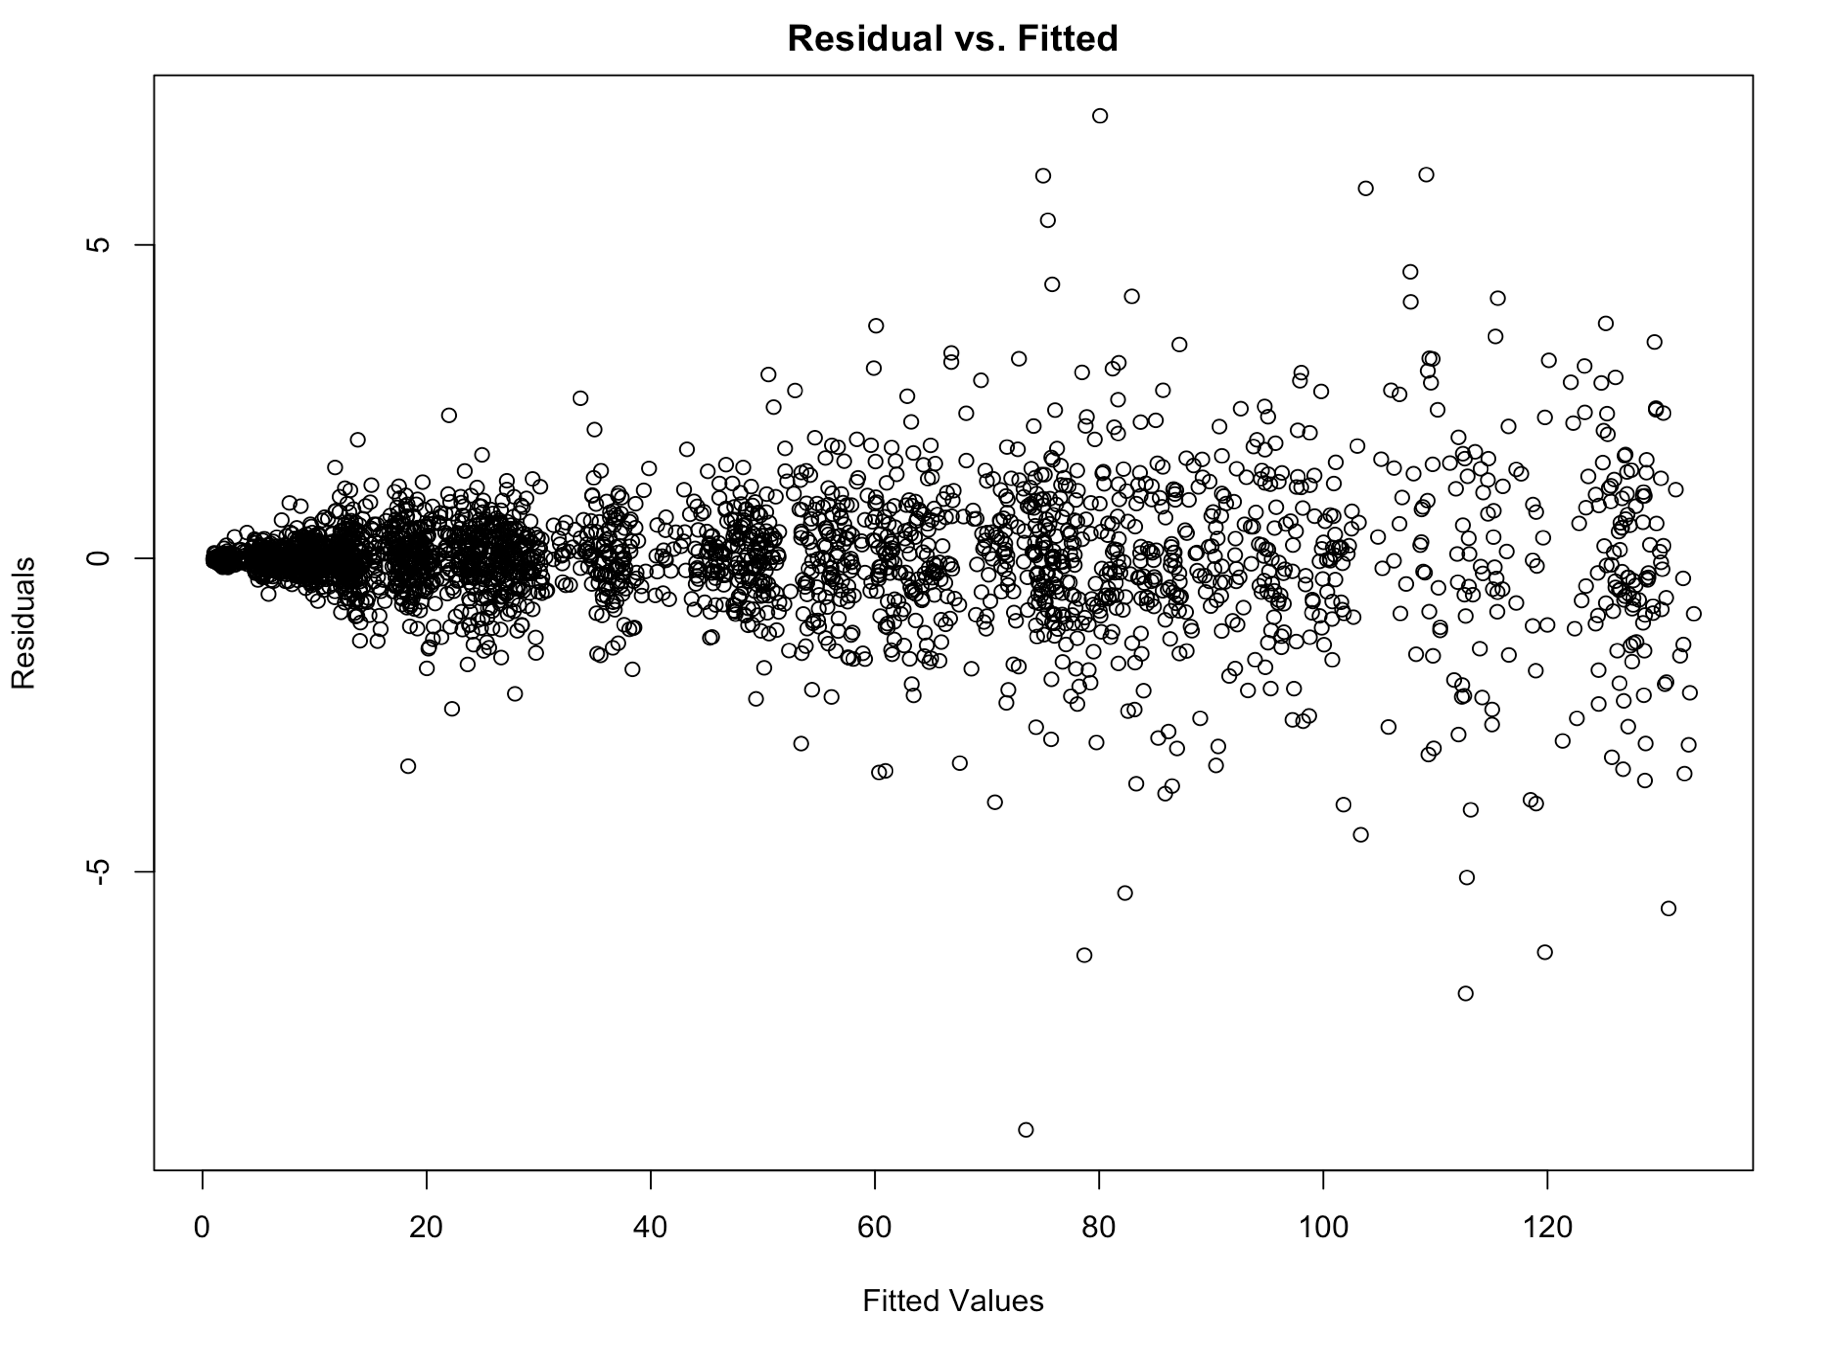
\includegraphics[width=90mm]{autoregressive_residual_vs_fitted.png}\end{center}

We tried to resolve the heteroscedascity issue by implementing a Weighted Least Squares autoregressive model but the results remained the same (see Appendix for full code and plot comparison). After some research, it turns out that this is an irreducible property of the autoregressive model because the data is serially correlated. We realized that we needed something better than directly modelling the price. Hence we decided to directly model the return which, to re-iterate, is defined as $ret.AAPL_i = \frac{AAPL_i - AAPL_{i-1}}{AAPL_{i-1}}$.

Correlation between the coefficients was also expected from the data. Since it is a time-series financial data set, we knew and verified that time is correlated to variables such as the Apple Stock Price and the $S \& P$ 500 Index. The detailed matrix can be found in the Appendix section. We decided that this wasn't too much of an issue since it is an inevitable part of any time-series data.

Moving on from the autoregressive model, we then considered automated model selecting using forward selection, backward elemination, and stepwise selection, from which we obtained the following models (full code in Appendix):


\textbf{Forward selection: } $Return = \beta_0 + \beta_1VIX + \beta_2AAPL2 + \beta_3AAPL + \beta_4SPGSCITR$

\textbf{Backward elimination: } $Return = \beta_0 + \beta_1AAPL + \beta_2VIX + \beta_3SPGSCITR + \beta_4AAPL2$

\textbf{Stepwise selection: } $Return = \beta_0 + \beta_1VIX + \beta_2AAPL2 + \beta_3AAPL + \beta_4SPGSCITR$


Interestingly, all selection methods returned the same model. Before we proceeded any further, we consulted with Prof. Zeng. After receiving helpful advice from the professor, we realized that since $Return$ is calculated as a function of $AAPL$ and $AAPL2$, the two variables cannot be included in the same model. We then adjusted the full model by excluding the variable $AAPL$, hence only keeping the previous-day price, and obtained the results below:


\textbf{Forward selection: } $ Return = \beta_0 + \beta_1VIX + \beta_2AAPL2 + \beta_3SPGSCITR + \beta_4EEM$

\textbf{Backward elimination: } $ Return = \beta_0 + \beta_1VIX + \beta_2AAPL2 + \beta_3SPGSCITR + \beta_4EEM$

\textbf{Stepwise selection: } $ Return = \beta_0 + \beta_1VIX + \beta_2AAPL2 + \beta_3SPGSCITR + \beta_4EEM$

We decided to further analyze this model in the model diagnostics section.

Additionally, we considered how the distribution of the independent variables could affect the model fit. Since both $VIX$ and $SPGSCITR$ had heavily skewed histograms, we decided to log-transform the variables to make the distributions resemble a normal curve and obtained the following model:
\textbf{Transformed model: } $ Return = \beta_0 + \beta_1(log(VIX)^{-2}) + \beta_2AAPL2 + \beta_3(log(SPGSCITR)) + \beta_4EEM$. This will be the second model to be discussed in the model diagnostics section.

\end{section}

\begin{section}{Model Diagnostics}

We first look into some diagnostic plots of the two models for the sake of residual analysis and outlier detection.

\begin{figure}[h]
\begin{subfigure}{.5\textwidth}
  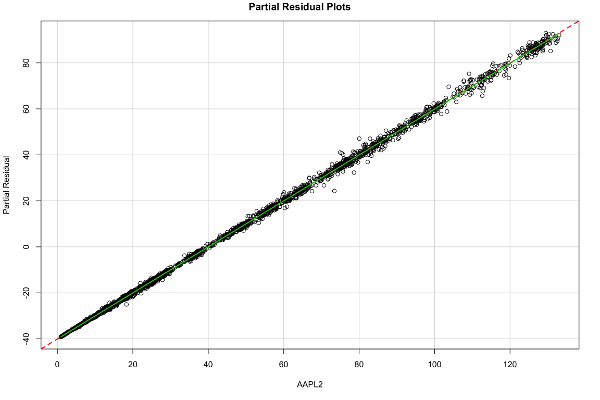
\includegraphics[width=90mm]{diagnostics/arm_covar_residuals.png}
  \caption{Autoregressive Model}
\end{subfigure}%
\begin{subfigure}{.5\textwidth}
  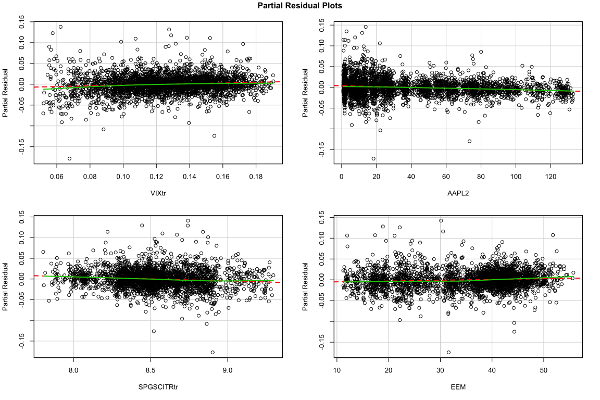
\includegraphics[width=90mm]{diagnostics/fm_covar_residuals.png}
  \caption{Automated Model}
\end{subfigure}
\end{figure}

There is a strong linear trend in the partial residual plot of the autoregressive model, and no deviation from the straight line. We see this trend with the covariates of the automated model as well, with only the `EEM` covariate and the log-transformed `VIX` displaying a small amount of deviation from the straight line. Hence, the assumption of linearity is satisfied for both models.

\begin{figure}[h]
\begin{subfigure}{.5\textwidth}
  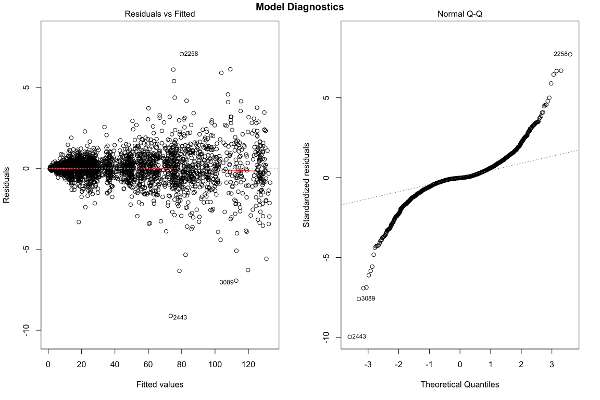
\includegraphics[width=90mm]{diagnostics/arm_model_plots.png}
  \caption{Autoregressive Model}
\end{subfigure}%
\begin{subfigure}{.5\textwidth}
  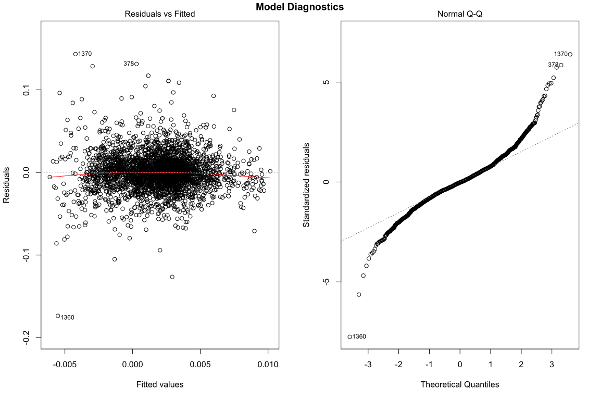
\includegraphics[width=90mm]{diagnostics/fm_model_plots.png}
  \caption{Automated Model}
\end{subfigure}
\end{figure}

The residuals of the autoregressive model are heterodastic as the plot of the residuals versus the fitted values has a fan-shaped pattern. In addition, the Q-Q plot of the residuals is heavy-tailed and exhibits curvature. In comparison, the plot of the residuals versus the fitted values of the automated model has more randomness than and lacks the fan-shaped pattern indicative of heterodasticity, and the Q-Q plot, while still being heavy-tailed, follows the linear trend more closely. Hence, the automated model produces errors that satisfy the assumption of constant error variance and that have non-normality that might be reasonably ignored, while the plots of the autoregressive model indicate that there are non-constant variances of the error and non-normality that we may be able to fix.


\begin{figure}[h]
\begin{subfigure}{.5\textwidth}
  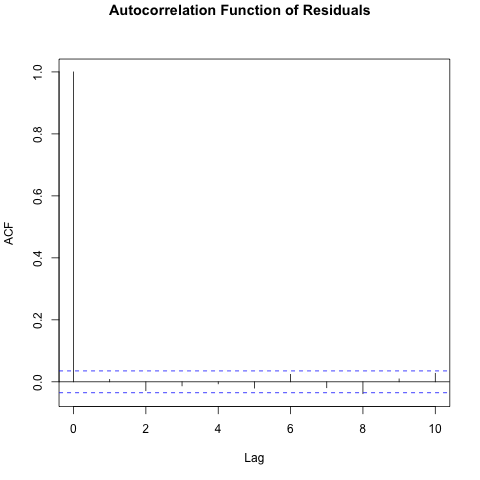
\includegraphics[width=90mm]{diagnostics/arm_acf_residuals.png}
  \caption{Autoregressive Model}
\end{subfigure}%
\begin{subfigure}{.5\textwidth}
  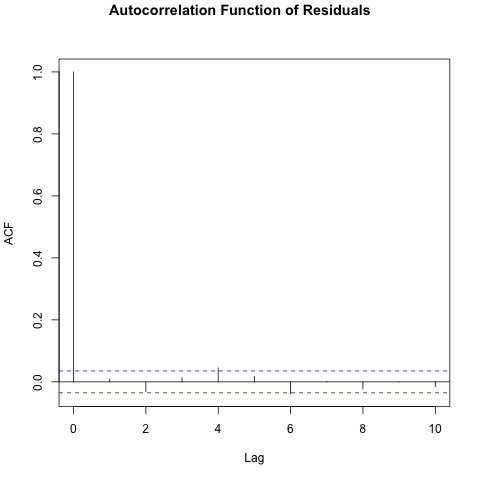
\includegraphics[width=90mm]{diagnostics/fm_acf_residuals.png}
  \caption{Automated Model}
\end{subfigure}
\end{figure}

We then looked into the last assumption of linear regression models: independence of the errors. As the stock data was time-series data and contained serial correlation, a scatterplot matrix was ruled out as a useful tool for detecting correlation. We instead considered ACF plots of the residuals, in combination with the results of the Durbin-Watson test. As can be seen in the ACF plots above, both models have explained away the autocorrelation in the residuals very well, as almost all of the sample correlations are within the limits. The results of the Durbin-Watson test on the models (shown in the table below) confirms this: for both models, the $p$-value of the test is high enough to accept the null hypothesis that there is no autocorrelation between the residuals.




\begin{table}[H]
\centering
\begin{tabular}{l|r|r}
\hline
  & Test Statistic & p-value\\
\hline
Autoregressive & 1.983123 & 0.5881467\\
\hline
Automated & 1.984218 & 0.6471835\\
\hline
\multicolumn{3}{l}{\textsuperscript{*} alternative: true autocorrelation is not}\\
\multicolumn{3}{l}{0}\\
\end{tabular}
\end{table}

The next concern we addressed was potential outliers and high-leverage cases. In both Cook's Distance plots below, there are no concerning observations that have a distance greater than 1, but most observations have a Cook's Distance greater than $p/n$, which is $0.0013$ and $0.00032$ for the automated and the autoregressive model, respectively. However, we see in both Residuals versus Leverage plots that there are no cases that are influential to the regression results. All points are well enough within the Cook's distance lines that said lines do not appear on either plot.

\begin{figure}[h]
\begin{subfigure}{.5\textwidth}
  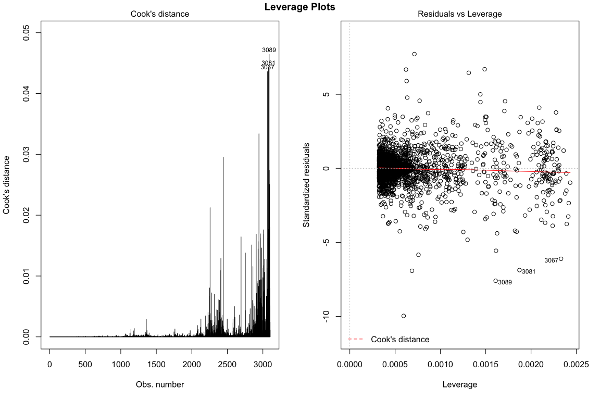
\includegraphics[width=90mm]{diagnostics/arm_leverage_plots.png}
  \caption{Autoregressive Model}
\end{subfigure}%
\begin{subfigure}{.5\textwidth}
  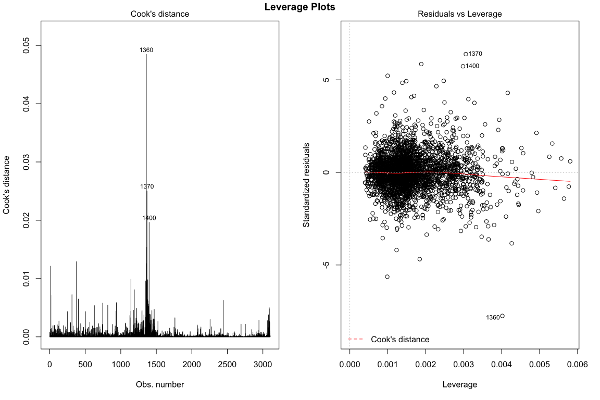
\includegraphics[width=90mm]{diagnostics/fm_leverage_plots.png}
  \caption{Automated Model}
\end{subfigure}
\end{figure}

Once we had performed residual analysis and outlier detection, we performed cross validation for the two models to determine if they were overfitting. The $k$-fold cross validation method was used - with $k=10$ - and the $RMSE$ over the 10 folds was calculated. For the sake of comparison, since the models have different dependent variables and hence different scales, the $RMSE$ had to be normalized by dividing it by the range of the observed values. We denote this calculation as the $NRMSE$. 

The autoregressive model has an $NRMSE$ of 0.00693, a value very close to 0, indicating that this model is a very good fit. While still being a well-fitted model, the automated model will generally produce less accurate predictions than the former model as it has a higher $NRMSE$ of 0.0706.

Add prediction analysis here

Based on our aforementioned results, the final model we decided to choose was the automated model, i.e. $ Return = \beta_0 + \beta_1(log(VIX)^{-2}) + \beta_2AAPL2 + \beta_3(log(SPGSCITR)) + \beta_4EEM$. While both models are well-fitted with most of the linear regression assumptions satisified and no significant outliers, the residuals of the automated model are homoodastic and are closer to normality than those of the autoregressive model. In addition, though the autoregressive model is less overfitted than the automated model (as measured by the $NRMSE$), it is not by a significant difference. The paramters estimates and confidence interval of the final model are displayed below in the table below.

\begin{table}[H]
\centering
\begin{tabular}{l|r|l}
\hline
  & Estimate & Intervals\\
\hline
(Intercept) & 0.0739397 & [0.0363, 0.1116]\\
\hline
VIXtr & 0.0855576 & [0.0549, 0.1162]\\
\hline
AAPL2 & -0.0000961 & [-1e-04, -1e-04]\\
\hline
SPGSCITRtr & -0.0100571 & [-0.0148, -0.0053]\\
\hline
EEM & 0.0001913 & [1e-04, 3e-04]\\
\hline
\end{tabular}
\end{table}

\end{section}

\begin{section}{Discussion}
\end{section}

\newpage

\begin{section}{Appendix}
Below is a collection of R code used in this report.
\end{section}

\subsubsection{Pre-process the data}\label{pre-process-the-data}

\begin{Shaded}
\begin{Highlighting}[]
\NormalTok{market_origin <-}\StringTok{ }\KeywordTok{read.csv}\NormalTok{(}\StringTok{"market_index_clean.csv"}\NormalTok{)}
\NormalTok{first <-}\StringTok{ }\NormalTok{market_origin[}\DecValTok{1}\NormalTok{,]}
\NormalTok{market <-}\StringTok{ }\NormalTok{market_origin[}\DecValTok{2}\OperatorTok{:}\DecValTok{3104}\NormalTok{,]}
\NormalTok{market}\OperatorTok{$}\NormalTok{AAPL2 <-}\StringTok{ }\NormalTok{market_origin[,}\StringTok{"AAPL"}\NormalTok{][}\DecValTok{1}\OperatorTok{:}\DecValTok{3103}\NormalTok{]}
\NormalTok{market}\OperatorTok{$}\NormalTok{Return <-}\StringTok{ }\NormalTok{(market}\OperatorTok{$}\NormalTok{AAPL }\OperatorTok{-}\StringTok{ }\NormalTok{market}\OperatorTok{$}\NormalTok{AAPL2)}\OperatorTok{/}\NormalTok{market}\OperatorTok{$}\NormalTok{AAPL2}
\end{Highlighting}
\end{Shaded}

\subsubsection{Full Model}\label{full-model}

\begin{Shaded}
\begin{Highlighting}[]
\KeywordTok{library}\NormalTok{(lubridate)}
\NormalTok{market}\OperatorTok{$}\NormalTok{Date <-}\StringTok{ }\NormalTok{market_origin}\OperatorTok{$}\NormalTok{Date[}\DecValTok{2}\OperatorTok{:}\DecValTok{3104}\NormalTok{]}
\NormalTok{date <-}\StringTok{ }\NormalTok{market}\OperatorTok{$}\NormalTok{Date}
\NormalTok{first <-}\StringTok{ }\NormalTok{date[}\DecValTok{1}\NormalTok{]}
\NormalTok{day <-}\StringTok{ }\KeywordTok{c}\NormalTok{()}
\ControlFlowTok{for}\NormalTok{(i }\ControlFlowTok{in} \DecValTok{1}\OperatorTok{:}\KeywordTok{length}\NormalTok{(date)) \{}
\NormalTok{  diff =}\StringTok{ }\KeywordTok{round}\NormalTok{(}\KeywordTok{difftime}\NormalTok{(date[i], first))}
\NormalTok{  day =}\StringTok{ }\KeywordTok{c}\NormalTok{(day, diff)}
\NormalTok{\}}
\NormalTok{market}\OperatorTok{$}\NormalTok{Date <-}\StringTok{ }\NormalTok{day}
\NormalTok{full_model <-}\StringTok{ }\KeywordTok{lm}\NormalTok{(Return}\OperatorTok{~}\NormalTok{., }\DataTypeTok{data =}\NormalTok{ market)}
\KeywordTok{summary}\NormalTok{(full_model)}
\end{Highlighting}
\end{Shaded}

\begin{verbatim}
## 
## Call:
## lm(formula = Return ~ ., data = market)
## 
## Residuals:
##       Min        1Q    Median        3Q       Max 
## -0.122225 -0.006376 -0.000258  0.005388  0.122985 
## 
## Coefficients:
##               Estimate Std. Error t value Pr(>|t|)    
## (Intercept)  2.004e-02  1.196e-02   1.675  0.09395 .  
## Date         9.523e-07  1.866e-06   0.510  0.60990    
## AAPL         1.652e-02  3.291e-04  50.193  < 2e-16 ***
## SPX         -2.934e-06  3.110e-06  -0.944  0.34544    
## VIX         -1.462e-04  5.296e-05  -2.760  0.00581 ** 
## SPGSCITR    -6.714e-07  3.345e-07  -2.007  0.04479 *  
## BNDGLB      -3.652e-05  4.143e-05  -0.882  0.37807    
## EEM          2.708e-05  5.865e-05   0.462  0.64431    
## AAPL2       -1.653e-02  3.287e-04 -50.287  < 2e-16 ***
## ---
## Signif. codes:  0 '***' 0.001 '**' 0.01 '*' 0.05 '.' 0.1 ' ' 1
## 
## Residual standard error: 0.01668 on 3094 degrees of freedom
## Multiple R-squared:  0.4559, Adjusted R-squared:  0.4545 
## F-statistic: 324.1 on 8 and 3094 DF,  p-value: < 2.2e-16
\end{verbatim}

\subsubsection{Null Model}\label{null-model}

\begin{Shaded}
\begin{Highlighting}[]
\NormalTok{null_model <-}\StringTok{ }\KeywordTok{lm}\NormalTok{(Return}\OperatorTok{~}\DecValTok{1}\NormalTok{, }\DataTypeTok{data =}\NormalTok{ market)}
\KeywordTok{summary}\NormalTok{(null_model)}
\end{Highlighting}
\end{Shaded}

\begin{verbatim}
## 
## Call:
## lm(formula = Return ~ 1, data = market)
## 
## Residuals:
##       Min        1Q    Median        3Q       Max 
## -0.181002 -0.011565 -0.000401  0.011553  0.137241 
## 
## Coefficients:
##              Estimate Std. Error t value Pr(>|t|)    
## (Intercept) 0.0018046  0.0004055    4.45  8.9e-06 ***
## ---
## Signif. codes:  0 '***' 0.001 '**' 0.01 '*' 0.05 '.' 0.1 ' ' 1
## 
## Residual standard error: 0.02259 on 3102 degrees of freedom
\end{verbatim}

\subsubsection{Autoregressive Model}\label{autoregressive-model}

\begin{Shaded}
\begin{Highlighting}[]
\NormalTok{autoregressive_model <-}\StringTok{ }\KeywordTok{lm}\NormalTok{(AAPL}\OperatorTok{~}\NormalTok{AAPL2, }\DataTypeTok{data =}\NormalTok{ market)}
\KeywordTok{plot}\NormalTok{(}\KeywordTok{fitted}\NormalTok{(autoregressive_model),}\KeywordTok{residuals}\NormalTok{(autoregressive_model), }
     \DataTypeTok{main =} \StringTok{"Residual vs. Fitted"}\NormalTok{, }\DataTypeTok{xlab =} \StringTok{"Fitted Values"}\NormalTok{, }\DataTypeTok{ylab =} \StringTok{"Residuals"}\NormalTok{)}
\end{Highlighting}
\end{Shaded}

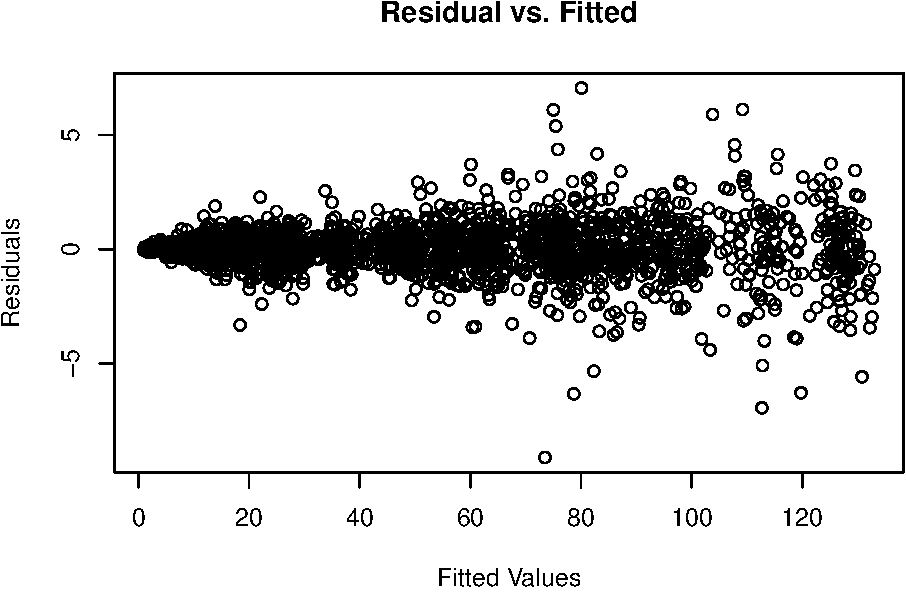
\includegraphics{report_files/figure-latex/unnamed-chunk-7-1.pdf}

\subsubsection{WLS Autoregressive Model}\label{wls-autoregressive-model}

\begin{Shaded}
\begin{Highlighting}[]
\NormalTok{wts <-}\DecValTok{1}\OperatorTok{/}\NormalTok{(}\KeywordTok{fitted}\NormalTok{(}\KeywordTok{lm}\NormalTok{(}\KeywordTok{abs}\NormalTok{(}\KeywordTok{residuals}\NormalTok{(autoregressive_model))}\OperatorTok{~}\KeywordTok{fitted}\NormalTok{(autoregressive_model)))}\OperatorTok{^}\DecValTok{2}\NormalTok{)}
\NormalTok{wls <-}\StringTok{ }\KeywordTok{lm}\NormalTok{(market}\OperatorTok{$}\NormalTok{AAPL}\OperatorTok{~}\NormalTok{market}\OperatorTok{$}\NormalTok{AAPL2, }\DataTypeTok{weights =}\NormalTok{ wts)}
\KeywordTok{par}\NormalTok{(}\DataTypeTok{mfrow=}\KeywordTok{c}\NormalTok{(}\DecValTok{1}\NormalTok{,}\DecValTok{2}\NormalTok{))}
\KeywordTok{plot}\NormalTok{(}\KeywordTok{fitted}\NormalTok{(autoregressive_model), autoregressive_model}\OperatorTok{$}\NormalTok{residuals, }
     \DataTypeTok{main=}\StringTok{"unweighted"}\NormalTok{, }\DataTypeTok{xlab =} \StringTok{"fitted"}\NormalTok{, }\DataTypeTok{ylab =} \StringTok{"residuals"}\NormalTok{)}
\KeywordTok{plot}\NormalTok{(}\KeywordTok{fitted}\NormalTok{(wls), wls}\OperatorTok{$}\NormalTok{residuals, }\DataTypeTok{main=}\StringTok{"weighted"}\NormalTok{, }\DataTypeTok{xlab =} \StringTok{"fitted"}\NormalTok{, }\DataTypeTok{ylab =} \StringTok{"residuals"}\NormalTok{)}
\end{Highlighting}
\end{Shaded}

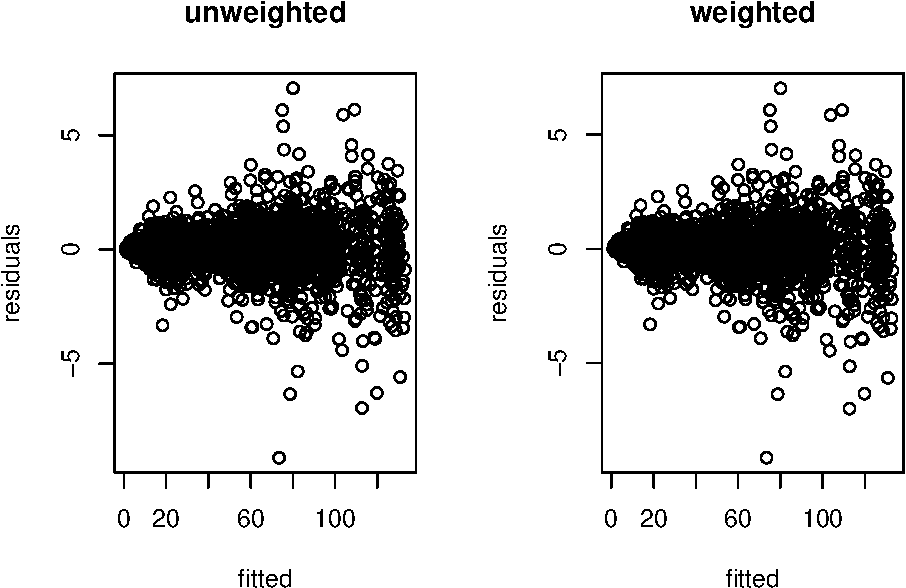
\includegraphics{report_files/figure-latex/unnamed-chunk-8-1.pdf}

There is no apparent difference between the weighted least squares and
the un-weighted autoregressive models.

\subsubsection{Correlation Matrix}\label{correlation-matrix}

\begin{Shaded}
\begin{Highlighting}[]
\KeywordTok{cor}\NormalTok{(market)}
\end{Highlighting}
\end{Shaded}

\begin{verbatim}
##                 Date        AAPL         SPX         VIX    SPGSCITR
## Date      1.00000000  0.93054238  0.69696343  0.01938577 -0.39587529
## AAPL      0.93054238  1.00000000  0.80227827 -0.15162359 -0.43263346
## SPX       0.69696343  0.80227827  1.00000000 -0.46846073 -0.12964526
## VIX       0.01938577 -0.15162359 -0.46846073  1.00000000 -0.13817311
## SPGSCITR -0.39587529 -0.43263346 -0.12964526 -0.13817311  1.00000000
## BNDGLB    0.97954886  0.91549333  0.61479422  0.01429116 -0.41500309
## EEM       0.69490012  0.56625441  0.52381985 -0.09933419  0.15774343
## AAPL2     0.93045589  0.99968333  0.80195192 -0.15030688 -0.43252990
## Return   -0.03966344 -0.02622066 -0.01334314 -0.07015138 -0.01064244
##               BNDGLB         EEM       AAPL2      Return
## Date      0.97954886  0.69490012  0.93045589 -0.03966344
## AAPL      0.91549333  0.56625441  0.99968333 -0.02622066
## SPX       0.61479422  0.52381985  0.80195192 -0.01334314
## VIX       0.01429116 -0.09933419 -0.15030688 -0.07015138
## SPGSCITR -0.41500309  0.15774343 -0.43252990 -0.01064244
## BNDGLB    1.00000000  0.67837773  0.91540368 -0.03817233
## EEM       0.67837773  1.00000000  0.56565038 -0.01874895
## AAPL2     0.91540368  0.56565038  1.00000000 -0.04313234
## Return   -0.03817233 -0.01874895 -0.04313234  1.00000000
\end{verbatim}

\subsubsection{Forward Selection}\label{forward-selection}

\begin{Shaded}
\begin{Highlighting}[]
\KeywordTok{step}\NormalTok{(null_model, }\DataTypeTok{scope =} \KeywordTok{list}\NormalTok{(}\DataTypeTok{upper=}\NormalTok{full_model), }\DataTypeTok{direction=}\StringTok{"forward"}\NormalTok{)}
\end{Highlighting}
\end{Shaded}

\begin{verbatim}
## Start:  AIC=-23521.04
## Return ~ 1
## 
##            Df Sum of Sq    RSS    AIC
## + VIX       1 0.0077908 1.5753 -23534
## + AAPL2     1 0.0029452 1.5801 -23525
## + Date      1 0.0024905 1.5806 -23524
## + BNDGLB    1 0.0023068 1.5808 -23524
## + AAPL      1 0.0010884 1.5820 -23521
## <none>                  1.5831 -23521
## + EEM       1 0.0005565 1.5825 -23520
## + SPX       1 0.0002819 1.5828 -23520
## + SPGSCITR  1 0.0001793 1.5829 -23519
## 
## Step:  AIC=-23534.35
## Return ~ VIX
## 
##            Df Sum of Sq    RSS    AIC
## + AAPL2     1 0.0046666 1.5706 -23542
## + SPX       1 0.0043302 1.5710 -23541
## + Date      1 0.0023235 1.5730 -23537
## + AAPL      1 0.0022012 1.5731 -23537
## + BNDGLB    1 0.0021876 1.5731 -23537
## + EEM       1 0.0010575 1.5742 -23534
## <none>                  1.5753 -23534
## + SPGSCITR  1 0.0006674 1.5746 -23534
## 
## Step:  AIC=-23541.56
## Return ~ VIX + AAPL2
## 
##            Df Sum of Sq     RSS    AIC
## + AAPL      1   0.70697 0.86367 -25395
## + SPGSCITR  1   0.00420 1.56644 -23548
## + Date      1   0.00245 1.56819 -23544
## + BNDGLB    1   0.00200 1.56864 -23544
## <none>                  1.57064 -23542
## + SPX       1   0.00025 1.57039 -23540
## + EEM       1   0.00005 1.57059 -23540
## 
## Step:  AIC=-25395.29
## Return ~ VIX + AAPL2 + AAPL
## 
##            Df  Sum of Sq     RSS    AIC
## + SPGSCITR  1 0.00201222 0.86166 -25400
## + EEM       1 0.00057998 0.86309 -25395
## <none>                   0.86367 -25395
## + SPX       1 0.00049664 0.86318 -25395
## + Date      1 0.00014064 0.86353 -25394
## + BNDGLB    1 0.00007249 0.86360 -25394
## 
## Step:  AIC=-25400.53
## Return ~ VIX + AAPL2 + AAPL + SPGSCITR
## 
##          Df  Sum of Sq     RSS    AIC
## <none>                 0.86166 -25400
## + SPX     1 5.4468e-05 0.86161 -25399
## + BNDGLB  1 4.5295e-05 0.86161 -25399
## + Date    1 3.2010e-05 0.86163 -25399
## + EEM     1 7.7700e-07 0.86166 -25398
\end{verbatim}

\begin{verbatim}
## 
## Call:
## lm(formula = Return ~ VIX + AAPL2 + AAPL + SPGSCITR, data = market)
## 
## Coefficients:
## (Intercept)          VIX        AAPL2         AAPL     SPGSCITR  
##   8.923e-03   -1.223e-04   -1.655e-02    1.650e-02   -6.748e-07
\end{verbatim}

\begin{Shaded}
\begin{Highlighting}[]
\KeywordTok{summary}\NormalTok{(}\KeywordTok{lm}\NormalTok{(}\DataTypeTok{formula =}\NormalTok{ Return }\OperatorTok{~}\StringTok{ }\NormalTok{VIX }\OperatorTok{+}\StringTok{ }\NormalTok{AAPL2 }\OperatorTok{+}\StringTok{ }\NormalTok{AAPL }\OperatorTok{+}\StringTok{ }\NormalTok{SPGSCITR, }\DataTypeTok{data =}\NormalTok{ market))}
\end{Highlighting}
\end{Shaded}

\begin{verbatim}
## 
## Call:
## lm(formula = Return ~ VIX + AAPL2 + AAPL + SPGSCITR, data = market)
## 
## Residuals:
##       Min        1Q    Median        3Q       Max 
## -0.122432 -0.006258 -0.000422  0.005541  0.122853 
## 
## Coefficients:
##               Estimate Std. Error t value Pr(>|t|)    
## (Intercept)  8.923e-03  1.833e-03   4.868 1.19e-06 ***
## VIX         -1.223e-04  3.389e-05  -3.609 0.000313 ***
## AAPL2       -1.655e-02  3.279e-04 -50.473  < 2e-16 ***
## AAPL         1.650e-02  3.279e-04  50.338  < 2e-16 ***
## SPGSCITR    -6.748e-07  2.509e-07  -2.690 0.007189 ** 
## ---
## Signif. codes:  0 '***' 0.001 '**' 0.01 '*' 0.05 '.' 0.1 ' ' 1
## 
## Residual standard error: 0.01668 on 3098 degrees of freedom
## Multiple R-squared:  0.4557, Adjusted R-squared:  0.455 
## F-statistic: 648.5 on 4 and 3098 DF,  p-value: < 2.2e-16
\end{verbatim}

\subsubsection{Backward Elimination}\label{backward-elimination}

\begin{Shaded}
\begin{Highlighting}[]
\KeywordTok{step}\NormalTok{(full_model, }\DataTypeTok{scope =} \KeywordTok{list}\NormalTok{(}\DataTypeTok{lower=}\NormalTok{null_model), }\DataTypeTok{direction=}\StringTok{"backward"}\NormalTok{)}
\end{Highlighting}
\end{Shaded}

\begin{verbatim}
## Start:  AIC=-25393.75
## Return ~ Date + AAPL + SPX + VIX + SPGSCITR + BNDGLB + EEM + 
##     AAPL2
## 
##            Df Sum of Sq     RSS    AIC
## - EEM       1   0.00006 0.86138 -25396
## - Date      1   0.00007 0.86139 -25396
## - BNDGLB    1   0.00022 0.86154 -25395
## - SPX       1   0.00025 0.86157 -25395
## <none>                  0.86132 -25394
## - SPGSCITR  1   0.00112 0.86244 -25392
## - VIX       1   0.00212 0.86344 -25388
## - AAPL      1   0.70133 1.56265 -23547
## - AAPL2     1   0.70397 1.56529 -23542
## 
## Step:  AIC=-25395.53
## Return ~ Date + AAPL + SPX + VIX + SPGSCITR + BNDGLB + AAPL2
## 
##            Df Sum of Sq     RSS    AIC
## - Date      1   0.00011 0.86149 -25397
## - BNDGLB    1   0.00019 0.86157 -25397
## - SPX       1   0.00023 0.86161 -25397
## <none>                  0.86138 -25396
## - SPGSCITR  1   0.00126 0.86264 -25393
## - VIX       1   0.00226 0.86365 -25389
## - AAPL      1   0.70153 1.56291 -23549
## - AAPL2     1   0.70584 1.56722 -23540
## 
## Step:  AIC=-25397.13
## Return ~ AAPL + SPX + VIX + SPGSCITR + BNDGLB + AAPL2
## 
##            Df Sum of Sq     RSS    AIC
## - BNDGLB    1   0.00011 0.86161 -25399
## - SPX       1   0.00012 0.86161 -25399
## <none>                  0.86149 -25397
## - SPGSCITR  1   0.00136 0.86286 -25394
## - VIX       1   0.00273 0.86422 -25389
## - AAPL      1   0.70192 1.56341 -23550
## - AAPL2     1   0.70725 1.56874 -23539
## 
## Step:  AIC=-25398.72
## Return ~ AAPL + SPX + VIX + SPGSCITR + AAPL2
## 
##            Df Sum of Sq     RSS    AIC
## - SPX       1   0.00005 0.86166 -25400
## <none>                  0.86161 -25399
## - SPGSCITR  1   0.00157 0.86318 -25395
## - VIX       1   0.00293 0.86453 -25390
## - AAPL      1   0.70478 1.56639 -23546
## - AAPL2     1   0.70759 1.56919 -23540
## 
## Step:  AIC=-25400.53
## Return ~ AAPL + VIX + SPGSCITR + AAPL2
## 
##            Df Sum of Sq     RSS    AIC
## <none>                  0.86166 -25400
## - SPGSCITR  1   0.00201 0.86367 -25395
## - VIX       1   0.00362 0.86528 -25390
## - AAPL      1   0.70478 1.56644 -23548
## - AAPL2     1   0.70856 1.57022 -23540
\end{verbatim}

\begin{verbatim}
## 
## Call:
## lm(formula = Return ~ AAPL + VIX + SPGSCITR + AAPL2, data = market)
## 
## Coefficients:
## (Intercept)         AAPL          VIX     SPGSCITR        AAPL2  
##   8.923e-03    1.650e-02   -1.223e-04   -6.748e-07   -1.655e-02
\end{verbatim}

\begin{Shaded}
\begin{Highlighting}[]
\KeywordTok{summary}\NormalTok{(}\KeywordTok{lm}\NormalTok{(}\DataTypeTok{formula =}\NormalTok{ Return }\OperatorTok{~}\StringTok{ }\NormalTok{AAPL }\OperatorTok{+}\StringTok{ }\NormalTok{VIX }\OperatorTok{+}\StringTok{ }\NormalTok{SPGSCITR }\OperatorTok{+}\StringTok{ }\NormalTok{AAPL2, }\DataTypeTok{data =}\NormalTok{ market))}
\end{Highlighting}
\end{Shaded}

\begin{verbatim}
## 
## Call:
## lm(formula = Return ~ AAPL + VIX + SPGSCITR + AAPL2, data = market)
## 
## Residuals:
##       Min        1Q    Median        3Q       Max 
## -0.122432 -0.006258 -0.000422  0.005541  0.122853 
## 
## Coefficients:
##               Estimate Std. Error t value Pr(>|t|)    
## (Intercept)  8.923e-03  1.833e-03   4.868 1.19e-06 ***
## AAPL         1.650e-02  3.279e-04  50.338  < 2e-16 ***
## VIX         -1.223e-04  3.389e-05  -3.609 0.000313 ***
## SPGSCITR    -6.748e-07  2.509e-07  -2.690 0.007189 ** 
## AAPL2       -1.655e-02  3.279e-04 -50.473  < 2e-16 ***
## ---
## Signif. codes:  0 '***' 0.001 '**' 0.01 '*' 0.05 '.' 0.1 ' ' 1
## 
## Residual standard error: 0.01668 on 3098 degrees of freedom
## Multiple R-squared:  0.4557, Adjusted R-squared:  0.455 
## F-statistic: 648.5 on 4 and 3098 DF,  p-value: < 2.2e-16
\end{verbatim}

\subsubsection{Stepwise Selection}\label{stepwise-selection}

\begin{Shaded}
\begin{Highlighting}[]
\KeywordTok{step}\NormalTok{(null_model, }\DataTypeTok{scope =} \KeywordTok{list}\NormalTok{(}\DataTypeTok{upper=}\NormalTok{full_model), }\DataTypeTok{direction=}\StringTok{"both"}\NormalTok{)}
\end{Highlighting}
\end{Shaded}

\begin{verbatim}
## Start:  AIC=-23521.04
## Return ~ 1
## 
##            Df Sum of Sq    RSS    AIC
## + VIX       1 0.0077908 1.5753 -23534
## + AAPL2     1 0.0029452 1.5801 -23525
## + Date      1 0.0024905 1.5806 -23524
## + BNDGLB    1 0.0023068 1.5808 -23524
## + AAPL      1 0.0010884 1.5820 -23521
## <none>                  1.5831 -23521
## + EEM       1 0.0005565 1.5825 -23520
## + SPX       1 0.0002819 1.5828 -23520
## + SPGSCITR  1 0.0001793 1.5829 -23519
## 
## Step:  AIC=-23534.35
## Return ~ VIX
## 
##            Df Sum of Sq    RSS    AIC
## + AAPL2     1 0.0046666 1.5706 -23542
## + SPX       1 0.0043302 1.5710 -23541
## + Date      1 0.0023235 1.5730 -23537
## + AAPL      1 0.0022012 1.5731 -23537
## + BNDGLB    1 0.0021876 1.5731 -23537
## + EEM       1 0.0010575 1.5742 -23534
## <none>                  1.5753 -23534
## + SPGSCITR  1 0.0006674 1.5746 -23534
## - VIX       1 0.0077908 1.5831 -23521
## 
## Step:  AIC=-23541.56
## Return ~ VIX + AAPL2
## 
##            Df Sum of Sq     RSS    AIC
## + AAPL      1   0.70697 0.86367 -25395
## + SPGSCITR  1   0.00420 1.56644 -23548
## + Date      1   0.00245 1.56819 -23544
## + BNDGLB    1   0.00200 1.56864 -23544
## <none>                  1.57064 -23542
## + SPX       1   0.00025 1.57039 -23540
## + EEM       1   0.00005 1.57059 -23540
## - AAPL2     1   0.00467 1.57531 -23534
## - VIX       1   0.00951 1.58015 -23525
## 
## Step:  AIC=-25395.29
## Return ~ VIX + AAPL2 + AAPL
## 
##            Df Sum of Sq     RSS    AIC
## + SPGSCITR  1   0.00201 0.86166 -25400
## + EEM       1   0.00058 0.86309 -25395
## <none>                  0.86367 -25395
## + SPX       1   0.00050 0.86318 -25395
## + Date      1   0.00014 0.86353 -25394
## + BNDGLB    1   0.00007 0.86360 -25394
## - VIX       1   0.00263 0.86630 -25388
## - AAPL      1   0.70697 1.57064 -23542
## - AAPL2     1   0.70943 1.57310 -23537
## 
## Step:  AIC=-25400.53
## Return ~ VIX + AAPL2 + AAPL + SPGSCITR
## 
##            Df Sum of Sq     RSS    AIC
## <none>                  0.86166 -25400
## + SPX       1   0.00005 0.86161 -25399
## + BNDGLB    1   0.00005 0.86161 -25399
## + Date      1   0.00003 0.86163 -25399
## + EEM       1   0.00000 0.86166 -25398
## - SPGSCITR  1   0.00201 0.86367 -25395
## - VIX       1   0.00362 0.86528 -25390
## - AAPL      1   0.70478 1.56644 -23548
## - AAPL2     1   0.70856 1.57022 -23540
\end{verbatim}

\begin{verbatim}
## 
## Call:
## lm(formula = Return ~ VIX + AAPL2 + AAPL + SPGSCITR, data = market)
## 
## Coefficients:
## (Intercept)          VIX        AAPL2         AAPL     SPGSCITR  
##   8.923e-03   -1.223e-04   -1.655e-02    1.650e-02   -6.748e-07
\end{verbatim}

\subsubsection{Forward Selection without
AAPL}\label{forward-selection-without-aapl}

\begin{Shaded}
\begin{Highlighting}[]
\NormalTok{full_model <-}\StringTok{ }\KeywordTok{lm}\NormalTok{(Return}\OperatorTok{~}\NormalTok{SPX}\OperatorTok{+}\NormalTok{VIX}\OperatorTok{+}\NormalTok{SPGSCITR}\OperatorTok{+}\NormalTok{BNDGLB}\OperatorTok{+}\NormalTok{EEM}\OperatorTok{+}\NormalTok{AAPL2, }\DataTypeTok{data =}\NormalTok{ market)}
\KeywordTok{step}\NormalTok{(null_model, }\DataTypeTok{scope =} \KeywordTok{list}\NormalTok{(}\DataTypeTok{upper=}\NormalTok{full_model), }\DataTypeTok{direction=}\StringTok{"forward"}\NormalTok{)}
\end{Highlighting}
\end{Shaded}

\begin{verbatim}
## Start:  AIC=-23521.04
## Return ~ 1
## 
##            Df Sum of Sq    RSS    AIC
## + VIX       1 0.0077908 1.5753 -23534
## + AAPL2     1 0.0029452 1.5801 -23525
## + BNDGLB    1 0.0023068 1.5808 -23524
## <none>                  1.5831 -23521
## + EEM       1 0.0005565 1.5825 -23520
## + SPX       1 0.0002819 1.5828 -23520
## + SPGSCITR  1 0.0001793 1.5829 -23519
## 
## Step:  AIC=-23534.35
## Return ~ VIX
## 
##            Df Sum of Sq    RSS    AIC
## + AAPL2     1 0.0046666 1.5706 -23542
## + SPX       1 0.0043302 1.5710 -23541
## + BNDGLB    1 0.0021876 1.5731 -23537
## + EEM       1 0.0010575 1.5742 -23534
## <none>                  1.5753 -23534
## + SPGSCITR  1 0.0006674 1.5746 -23534
## 
## Step:  AIC=-23541.56
## Return ~ VIX + AAPL2
## 
##            Df Sum of Sq    RSS    AIC
## + SPGSCITR  1 0.0042022 1.5664 -23548
## + BNDGLB    1 0.0019985 1.5686 -23544
## <none>                  1.5706 -23542
## + SPX       1 0.0002472 1.5704 -23540
## + EEM       1 0.0000477 1.5706 -23540
## 
## Step:  AIC=-23547.87
## Return ~ VIX + AAPL2 + SPGSCITR
## 
##          Df  Sum of Sq    RSS    AIC
## + EEM     1 0.00261906 1.5638 -23551
## + BNDGLB  1 0.00222991 1.5642 -23550
## <none>                 1.5664 -23548
## + SPX     1 0.00004699 1.5664 -23546
## 
## Step:  AIC=-23551.06
## Return ~ VIX + AAPL2 + SPGSCITR + EEM
## 
##          Df  Sum of Sq    RSS    AIC
## <none>                 1.5638 -23551
## + BNDGLB  1 0.00040528 1.5634 -23550
## + SPX     1 0.00007224 1.5637 -23549
\end{verbatim}

\begin{verbatim}
## 
## Call:
## lm(formula = Return ~ VIX + AAPL2 + SPGSCITR + EEM, data = market)
## 
## Coefficients:
## (Intercept)          VIX        AAPL2     SPGSCITR          EEM  
##   1.268e-02   -2.362e-04   -8.062e-05   -1.484e-06    1.323e-04
\end{verbatim}

\subsubsection{Backward Elimination without
AAPL}\label{backward-elimination-without-aapl}

\begin{Shaded}
\begin{Highlighting}[]
\KeywordTok{step}\NormalTok{(full_model, }\DataTypeTok{scope =} \KeywordTok{list}\NormalTok{(}\DataTypeTok{lower=}\NormalTok{null_model), }\DataTypeTok{direction=}\StringTok{"backward"}\NormalTok{)}
\end{Highlighting}
\end{Shaded}

\begin{verbatim}
## Start:  AIC=-23548.72
## Return ~ SPX + VIX + SPGSCITR + BNDGLB + EEM + AAPL2
## 
##            Df Sum of Sq    RSS    AIC
## - SPX       1 0.0004317 1.5634 -23550
## - EEM       1 0.0004341 1.5634 -23550
## - BNDGLB    1 0.0007647 1.5637 -23549
## <none>                  1.5630 -23549
## - AAPL2     1 0.0039998 1.5670 -23543
## - SPGSCITR  1 0.0051524 1.5681 -23540
## - VIX       1 0.0087690 1.5717 -23533
## 
## Step:  AIC=-23549.87
## Return ~ VIX + SPGSCITR + BNDGLB + EEM + AAPL2
## 
##            Df Sum of Sq    RSS    AIC
## - BNDGLB    1 0.0004053 1.5638 -23551
## - EEM       1 0.0007944 1.5642 -23550
## <none>                  1.5634 -23550
## - SPGSCITR  1 0.0048344 1.5682 -23542
## - AAPL2     1 0.0054852 1.5689 -23541
## - VIX       1 0.0130706 1.5765 -23526
## 
## Step:  AIC=-23551.06
## Return ~ VIX + SPGSCITR + EEM + AAPL2
## 
##            Df Sum of Sq    RSS    AIC
## <none>                  1.5638 -23551
## - EEM       1 0.0026191 1.5664 -23548
## - SPGSCITR  1 0.0067735 1.5706 -23540
## - AAPL2     1 0.0099762 1.5738 -23533
## - VIX       1 0.0133247 1.5771 -23527
\end{verbatim}

\begin{verbatim}
## 
## Call:
## lm(formula = Return ~ VIX + SPGSCITR + EEM + AAPL2, data = market)
## 
## Coefficients:
## (Intercept)          VIX     SPGSCITR          EEM        AAPL2  
##   1.268e-02   -2.362e-04   -1.484e-06    1.323e-04   -8.062e-05
\end{verbatim}

\subsubsection{Stepwise Selection without
AAPL}\label{stepwise-selection-without-aapl}

\begin{Shaded}
\begin{Highlighting}[]
\KeywordTok{step}\NormalTok{(null_model, }\DataTypeTok{scope =} \KeywordTok{list}\NormalTok{(}\DataTypeTok{upper=}\NormalTok{full_model), }\DataTypeTok{direction=}\StringTok{"both"}\NormalTok{)}
\end{Highlighting}
\end{Shaded}

\begin{verbatim}
## Start:  AIC=-23521.04
## Return ~ 1
## 
##            Df Sum of Sq    RSS    AIC
## + VIX       1 0.0077908 1.5753 -23534
## + AAPL2     1 0.0029452 1.5801 -23525
## + BNDGLB    1 0.0023068 1.5808 -23524
## <none>                  1.5831 -23521
## + EEM       1 0.0005565 1.5825 -23520
## + SPX       1 0.0002819 1.5828 -23520
## + SPGSCITR  1 0.0001793 1.5829 -23519
## 
## Step:  AIC=-23534.35
## Return ~ VIX
## 
##            Df Sum of Sq    RSS    AIC
## + AAPL2     1 0.0046666 1.5706 -23542
## + SPX       1 0.0043302 1.5710 -23541
## + BNDGLB    1 0.0021876 1.5731 -23537
## + EEM       1 0.0010575 1.5742 -23534
## <none>                  1.5753 -23534
## + SPGSCITR  1 0.0006674 1.5746 -23534
## - VIX       1 0.0077908 1.5831 -23521
## 
## Step:  AIC=-23541.56
## Return ~ VIX + AAPL2
## 
##            Df Sum of Sq    RSS    AIC
## + SPGSCITR  1 0.0042022 1.5664 -23548
## + BNDGLB    1 0.0019985 1.5686 -23544
## <none>                  1.5706 -23542
## + SPX       1 0.0002472 1.5704 -23540
## + EEM       1 0.0000477 1.5706 -23540
## - AAPL2     1 0.0046666 1.5753 -23534
## - VIX       1 0.0095122 1.5801 -23525
## 
## Step:  AIC=-23547.87
## Return ~ VIX + AAPL2 + SPGSCITR
## 
##            Df Sum of Sq    RSS    AIC
## + EEM       1 0.0026191 1.5638 -23551
## + BNDGLB    1 0.0022299 1.5642 -23550
## <none>                  1.5664 -23548
## + SPX       1 0.0000470 1.5664 -23546
## - SPGSCITR  1 0.0042022 1.5706 -23542
## - AAPL2     1 0.0082014 1.5746 -23534
## - VIX       1 0.0120427 1.5785 -23526
## 
## Step:  AIC=-23551.06
## Return ~ VIX + AAPL2 + SPGSCITR + EEM
## 
##            Df Sum of Sq    RSS    AIC
## <none>                  1.5638 -23551
## + BNDGLB    1 0.0004053 1.5634 -23550
## + SPX       1 0.0000722 1.5637 -23549
## - EEM       1 0.0026191 1.5664 -23548
## - SPGSCITR  1 0.0067735 1.5706 -23540
## - AAPL2     1 0.0099762 1.5738 -23533
## - VIX       1 0.0133247 1.5771 -23527
\end{verbatim}

\begin{verbatim}
## 
## Call:
## lm(formula = Return ~ VIX + AAPL2 + SPGSCITR + EEM, data = market)
## 
## Coefficients:
## (Intercept)          VIX        AAPL2     SPGSCITR          EEM  
##   1.268e-02   -2.362e-04   -8.062e-05   -1.484e-06    1.323e-04
\end{verbatim}

\subsubsection{Log-transformed model from stepwise selection
results}\label{log-transformed-model-from-stepwise-selection-results}

\begin{Shaded}
\begin{Highlighting}[]
\NormalTok{## note that the VIX needed to be raised to the -2, after the log transformation}
\NormalTok{##  in order to obtain a distribution close to the Gaussian curve}
\NormalTok{VIXtr <-}\StringTok{ }\KeywordTok{log}\NormalTok{(market}\OperatorTok{$}\NormalTok{VIX)}\OperatorTok{^-}\DecValTok{2}
\KeywordTok{hist}\NormalTok{(VIXtr)}
\end{Highlighting}
\end{Shaded}

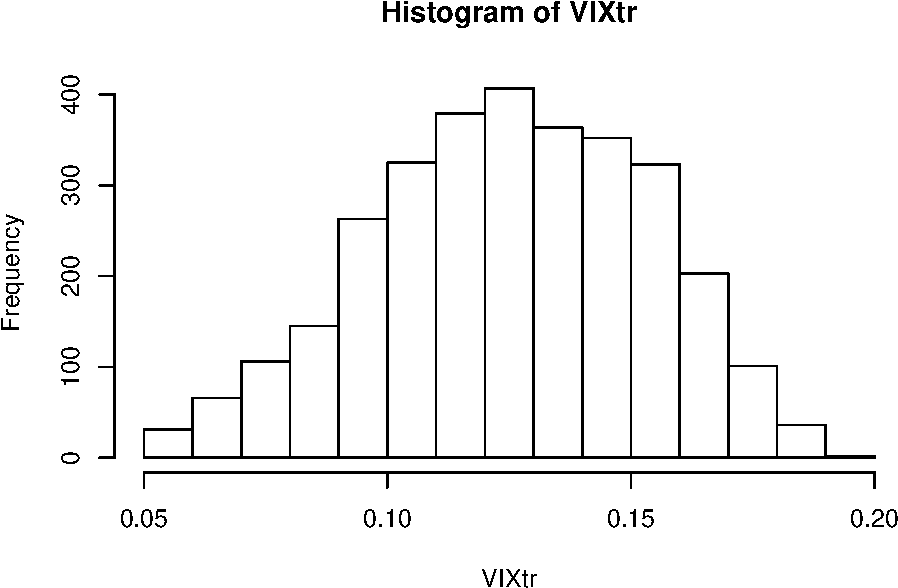
\includegraphics{report_files/figure-latex/unnamed-chunk-16-1.pdf}

\begin{Shaded}
\begin{Highlighting}[]
\NormalTok{SPGSCITRtr <-}\StringTok{ }\KeywordTok{log}\NormalTok{(market}\OperatorTok{$}\NormalTok{SPGSCITR)}
\KeywordTok{hist}\NormalTok{(SPGSCITRtr)}
\end{Highlighting}
\end{Shaded}

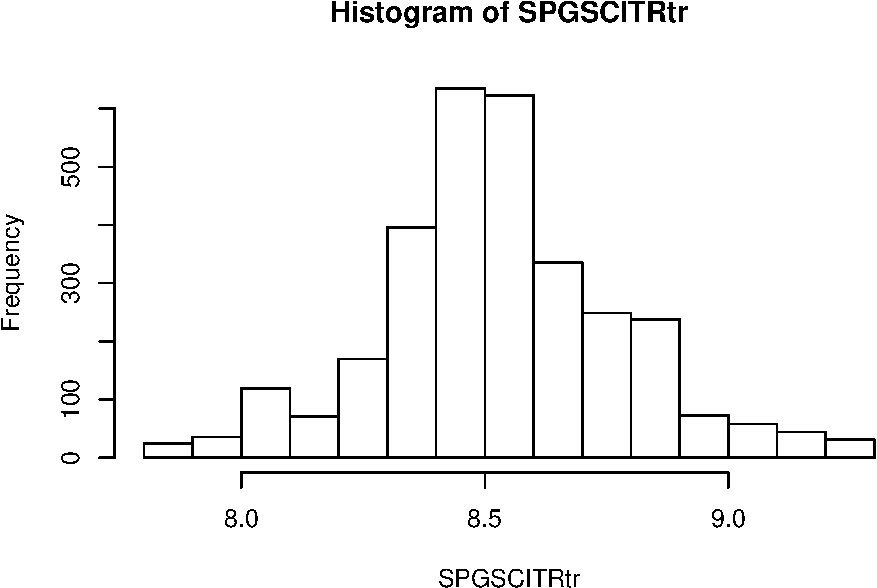
\includegraphics{report_files/figure-latex/unnamed-chunk-16-2.pdf}

\begin{Shaded}
\begin{Highlighting}[]
\NormalTok{transformed_model <-}\StringTok{ }\KeywordTok{lm}\NormalTok{(market}\OperatorTok{$}\NormalTok{Return}\OperatorTok{~}\NormalTok{VIXtr}\OperatorTok{+}\NormalTok{SPGSCITRtr}\OperatorTok{+}\NormalTok{market}\OperatorTok{$}\NormalTok{EEM}\OperatorTok{+}\NormalTok{market}\OperatorTok{$}\NormalTok{AAPL2)}
\KeywordTok{summary}\NormalTok{(transformed_model)}
\end{Highlighting}
\end{Shaded}

\begin{verbatim}
## 
## Call:
## lm(formula = market$Return ~ VIXtr + SPGSCITRtr + market$EEM + 
##     market$AAPL2)
## 
## Residuals:
##       Min        1Q    Median        3Q       Max 
## -0.173682 -0.011659 -0.000509  0.011447  0.143266 
## 
## Coefficients:
##                Estimate Std. Error t value Pr(>|t|)    
## (Intercept)   7.394e-02  1.922e-02   3.847 0.000122 ***
## VIXtr         8.556e-02  1.562e-02   5.478 4.66e-08 ***
## SPGSCITRtr   -1.006e-02  2.409e-03  -4.174 3.07e-05 ***
## market$EEM    1.913e-04  6.117e-05   3.127 0.001782 ** 
## market$AAPL2 -9.605e-05  1.958e-05  -4.906 9.80e-07 ***
## ---
## Signif. codes:  0 '***' 0.001 '**' 0.01 '*' 0.05 '.' 0.1 ' ' 1
## 
## Residual standard error: 0.02246 on 3098 degrees of freedom
## Multiple R-squared:  0.01312,    Adjusted R-squared:  0.01185 
## F-statistic:  10.3 on 4 and 3098 DF,  p-value: 2.764e-08
\end{verbatim}


\end{document}
